\chapter{Proofs}

\section{Luck more generally.}
Fundamentally, defining luck depends on a partial ordering of the elements of the probability space in question.  In a finite or countable space, this can be done just from the probability.  In larger spaces more topological structure is required:
\begin{equation}
\label{eq:less}
y < x \text{\ iff\ } \lim_{r \downarrow 0} \frac{p(B_r(x))}{p(B_r(y))} < 1 \,.
\end{equation}
Here, $p(S)$ denotes the probability of an outcome in $S \subseteq X$, and $B_\varepsilon(x) \subseteq X$ is the open ball of radius $r$ in the topology of $X$.

It is straightforward to prove the transitivity of (\ref{eq:less}).  Using this ordering, luck can be generalized as follows:
\index{Omega $\Omega$ ! definition (measure)}
\index{Omega $\Omega$ ! size $\abs{\Omega}$ (measure)}
\index{omega $\omega$ ! definition (measure)}
\index{omega $\omega$ ! size $\abs{\omega}$ (measure)}
\begin{align}
\Omega(x) &= \left\{ y \mid y < x \right\} \,, \\
|\Omega(x)| &= p(\Omega(x))  \,, \\
\omega(x) &= \left\{ y \mid y \nless x \andop x \nless y \right\} \,, \\
|\omega(x)| &= p(\omega(x)) \,, \\
\intertext{and}
\index{luck $L$ ! definition (measure)}
L(x) &= |\Omega(x)| + \frac{1}{2} |\omega(x)|\,.
\end{align}

\section{From the introduction}

\begin{theorem}{Range of Luck.} 
\label{thm:range}
For any probability space,
\begin{equation}
0 \leq L(x) \leq 1 \,.
\end{equation}

Proof.  From the definition, $L(x)=|\Omega(x)|+\frac{1}{2} |\omega(x)|$, which is clearly non-negative, and $\Omega(x)$ and $\omega(x)$ are disjoint subsets of the probability space.  Here the $| \cdot |$ notation is the measure of these sets in the probability space, and their union is at most the whole space, so $L(x) \leq |\Omega(x) \cup \omega(x)| \leq 1$.
\end{theorem}

\begin{theorem}{Lucky values.}
\label{thm:lucky}
If $L(x)$ is close to 1, then $p(x)$ is relatively small and most outcomes have a higher probability (you are lucky).

Proof.  Since $L(x)$ is close to 1, write $L(x)=1-\varepsilon(x)$, where $\varepsilon(x)$ is a small non-negative number.

First, since $\Omega(x)$ and $\omega(x)$ are disjoint subsets of the space of outcomes $X$, $|\Omega(x)|+|\omega(x)| \leq 1$, or 
\begin{equation*}
|\Omega(x)| \leq 1-|\omega(x)| \,.
\end{equation*}

Second, $L(x)=|\Omega(x)|+\frac{1}{2}|\omega(x)|$, which by the first inequality can be bounded as $1-\varepsilon(x)\leq  1-|\omega(x)|+\frac{1}{2}|\omega(x)|$, which can be rearranged as
\begin{equation*}
|\omega(x)| \leq 2 \varepsilon(x) \,.
\end{equation*}

Third, $|\Omega(x)|+\frac{1}{2}|\omega(x)| = 1-\varepsilon(x)$, or $|\Omega(x)|=1-\varepsilon(x)-\frac{1}{2}|\omega(x)|$, which by the second inequality,
\begin{equation}
|\Omega(x)| \geq 1-2 \varepsilon(x) \,.
\end{equation}
Thus at least a $1-2 \varepsilon(x)$ fraction of the probability space have a higher probability of occurring.
\end{theorem}

\begin{theorem}{Unlucky values.}
\label{thm:unlucky}
If $L(x)$ is close to 0, then $p(x)$ is comparatively large, and most outcomes would have a lower probability (you are unlucky).

Proof.  Since $L(x)$ is close to 0, write $L(x)=\varepsilon(x)$, where $\varepsilon(x)$ is a small non-negative number.

First, $L(x)=|\Omega(x)|+\frac{1}{2}|\omega(x)|$, so
\begin{equation*}
\omega(x) \leq 2\varepsilon(x) \,.
\end{equation*}

Second, $|\Omega(x)|+|\omega(x)|=|\Omega(x)|+\frac{1}{2}|\omega(x)|+\frac{1}{2}|\omega(x)| \leq 2\varepsilon(x)$, so
\begin{equation*}
|\Omega(x)|+|\omega(x)| \leq 2\varepsilon(x) \,.
\end{equation*}

Third, $|X-[\Omega(x) \cup \omega(x)]| \geq 1-|\Omega(x) \cup \omega(x)| \geq 1-2\varepsilon(x)$, or 
\begin{equation*}
|X-[\Omega(x) \cup \omega(x)]| \geq 1-2\varepsilon(x) \,.
\end{equation*}
Thus at least a $1-2 \varepsilon(x)$ fraction of the probability space have a lower probability of occurring.
\end{theorem}

\begin{theorem}{On average, luck is always 50:50.}
\label{thm:fifty}

\begin{equation*}
E(L)=\frac{1}{2} \,.
\end{equation*}

Proof.  This is an application of the next theorem where $f(L)=L$.
\end{theorem}

\begin{theorem}{Smooth uniformity - finite space $X$.}
\label{thm:smooth-uniformity}

$E(f(L))=\int_0^1 f(L) dL-\varepsilon$, where $|\varepsilon| \leq \max|f''| \cdot \max |\omega|^2 / 24$.

Since the definition of luck only depends on the probabilities of outcomes, it is natural to consider the set of equivalence classes $[x]$ from $[X]$ defined by equal probabilities: $[x]=\{y \mid p(y)=p(x) \}$.  

We also use the midpoint integration estimate:
\begin{equation*}
\int_{a}^{b} f(L) \, dL = (b-a)f(\frac{a+b}{2})+\frac{(b-a)^3}{24} f''(\xi), \text{where $a < \xi < b$.}
\end{equation*}

\begin{align}
\int_0^1 f(L) \, dL 
  &= \sum_{[x]} \int_{L([x])-\frac{1}{2}|\omega([x])|}^{L([x])+\frac{1}{2}|\omega([x])|} f(L) \, dL \,, \\
  &= \sum_{[x]} \left\{ |\omega([x])| f(L([x])) + \frac{|\omega([x])|^3}{24} f''(\xi_{[x]}) \right\} \,, \\
  &= \sum_{x} p(x) f(L(x)) - \varepsilon \,, \\
  &= E(f(L)) -\varepsilon \,, \\
\varepsilon 
\label{eq:midpointerror}
   &= \sum_{[x]} \frac{|\omega([x])|^3}{24} f''(\xi_{[x]}) \,, \\
 |\varepsilon| 
   &\leq \frac{1}{24} \max_{x} |\omega(x)|^2 \cdot \max_{0\leq L \leq 1} |f''(L)| \,.
\end{align}
\end{theorem}

\begin{theorem}{Best of luck - finite space $X$.}
\label{thm:best-uniformity}
The fact that the definition of luck samples the intervals in theorem \ref{thm:smooth-uniformity} at the centers.  This is by design and is the only choice that leads to a second-order error error ($f''$) with the following constraints:
\begin{itemize}
\item Luck is constant for constant probabilities: if $p(x)=p(y)$ then $L(x)=L(y)$.
\item Luck is increasing for decreasing probabilities: if $p(x)<p(y)$ then $L(x)>L(y)$.
\end{itemize}
\begin{align}
E(f(L)) &= \sum_x p(x) f(L(x)) \\
\intertext{using equality of luck for equal probabilities}
        &= \sum_{[x]} |\omega([x])| f(L([x]))
\end{align}
Optimizing this sum as a quadrature of $\int_0^1 f(L) \, dL$ is a classic question answered by the gauss points (centers of the intervals).  The fact that $L(x)$ is increasing orders the gauss points to our definition of luck.
\end{theorem}

\begin{theorem}{Moments - finite space $X$.}
\label{thm:moments}
For $p \geq 2$, $E(L^p)=1/(p+1)-\varepsilon$, $0 \leq \varepsilon \leq p \cdot (p-1) \max |\omega|^2/24$.

Proof.  This is an example of $f(L)=L^p$ with $p \geq 1$ in the theorem above, and noting that $f''(L)$ is non-negative, so $\varepsilon$ in (\ref{eq:midpointerror}) must be non-negative.
\end{theorem}

\begin{theorem}{Interval uniformity - finite space $X$.}
\label{thm:interval-uniformity}
For $0 \leq a \leq b \leq 1$, $E(L \in [a,b])=b-a - \varepsilon$, $|\varepsilon| \leq \max |\omega|$.

Proof.  Let $f(L)$ be the characteristic function for the closed interval $[a,b]$.
\begin{align}
b-a &=\int_0^1 f(L) \, dL  \\
  &= \sum_{[x]} \int_{L([x])-\frac{1}{2}|\omega([x])|}^{L([x])+\frac{1}{2}|\omega([x])|} f(L) \, dL \,, \\
  &= E(f(L)) + \varepsilon \,, \\
\varepsilon &= \sum_{[x]} \int_{L([x])-\frac{1}{2}|\omega([x])|}^{L([x])+\frac{1}{2}|\omega([x])|} (f(L)-f(L([x]))) \, dL \,.
\end{align}
Now in the sum that defines $\varepsilon$, there are at most 2 discontinuities in an otherwise constant 0, 1 or -1 integrand.  If none occur in an interval, that term is exactly zero.  If one occurs, the integrand is zero for at least $\frac{1}{2}$ of the interval, so that error is at most $\frac{1}{2}|\omega([x])|$, and can be only once more in one other interval (with the same kind of error).  And if 2 occur, they occur nowhere else and the error is bounded by $|\omega([x])|$.  In each case we have our theorem.
\end{theorem}

\section{From Normal}
The approximation (\ref{eq:normal-luck-approx}), i.e.,
\begin{equation*}
L \approx L_1 = \frac{1}{2}\left[1+\erf(|\sqrt{\Sigma^{-1}} (x-\mu)|-\sqrt{n-1/2})\right] \,,
\end{equation*}
mostly comes from a Taylor expansion of the log of the integrand in (\ref{eq:normal-luck-as-integral}).  This in fact results in the approximation,
\begin{equation*}
L \approx L_2 =\frac{1}{2}\left[1+\erf(|\sqrt{\Sigma^{-1}} (x-\mu)|-\sqrt{n})\right] \,.
\end{equation*}
The shift from $\sqrt{n}$ to $\sqrt{n-1/2}$ was a result of numerical experimentation, summarized in figure~\ref{fig:estluck}.  It shows $\max |L-L_1|$ is has a $4 \times$ smaller than $\max |L-L_2|$ for $4 \leq n \leq 100,000$.
\begin{figure}
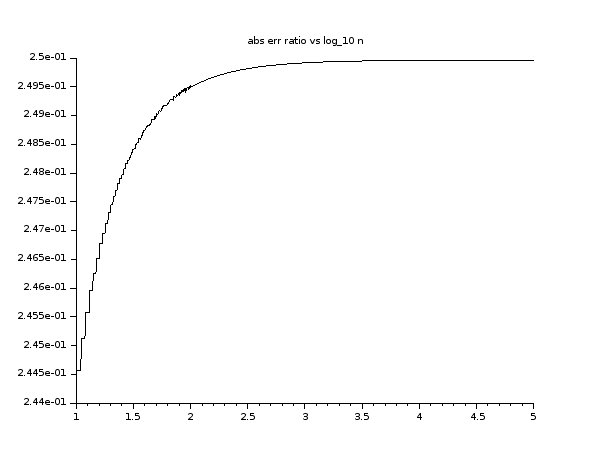
\includegraphics[width=0.75\linewidth]{img/estluck.png}
\caption[$\sqrt{n}$ vs $\sqrt{n-1/2}$]{This is a plot of $E(n)=\max_{0 \leq R \leq \infty}|L-L_1|/\max_{0 \leq R \leq \infty} |L-L_2|$ vs $\log_{10} n$. The $\sqrt{n-1/2}$-shift is always better than $\sqrt{n}$, and $4 \times$ better for $n \geq 4$ ($\log_{10} 4 \approx 0.6$).  The constant line is $1/4$ for reference.}
\label{fig:estluck}
\end{figure}

\section{From Computation}

In this section, we again consider only a finite probability space $X$ with $|X|$ elements $x_k$, $k=1,\ldots,|X|$ and probabilities $p_k=p(x_k)$.

Let $S=(s_1, \ldots, s_n)$ be $|S|$ independent samples taken from $X$.  We define an estimator for $L(x)$ as:
\begin{align*}
 \ell(x) = & \frac{1}{|S|} \left\{\text{\# of outcomes in S more probable than $x$}\right\}  \\
 & + \frac{1}{2|S|} \left\{\text{\# of outcomes in S equally probable to $x$}\right\} 
\end{align*}
We asserted that
\begin{align}
\label{eq:elmeanx}
E(\ell(x))&=L(x) \,. \\
\label{eq:elvariancex}
E([\ell(x)-L(x)]^2) &= \frac{1}{|S|} \left[L(x) \cdot (1-L(x)) -\frac{1}{4}|\omega(x)|\right] \,.
\end{align}

For the remainder of this section, we consider $x \in X$ to be a fixed choice, and so drop the $\cdot (x)$ functional notation, which would otherwise pepper every equation.  This way (\ref{eq:elmeanx}-\ref{eq:elvariancex}) becomes
\begin{align}
\label{eq:elmean}
E(\ell)&=L \,. \\
\label{eq:elvariance}
E([\ell-L]^2) &= \frac{1}{|S|} \left[L \cdot (1-L) -\frac{1}{4}|\omega|\right] \,
\end{align}
The point of this section is to work out the details of these facts.

The definition of $\ell$ does not depend on the ordering of the sample $S$, so the vector of counts $(c_1,\ldots,c_{|X|})$ is equivalent information about the sample for our purposes.  We define $c$ as the vector of counts of elements in $S$, so that $x_k$ occurs $c_k$ times in the sample $S$.

The probability of obtaining a sample counts $c$ is given by the multinomial distribution
\begin{equation}
P(c)=\left(\begin{array}{c} n \\ c \end{array}\right) p^c 
  = \frac{n!}{c_1! \cdot \cdots \cdot c_{|X|}!} p_1^{c_1} \cdots p_{|X|}^{c_{|X|}} \,, \text{where $n=\sum c=|S|$.}
\end{equation}
Here are some well-known moments of the multinomial distribution (the sum is over all samples with $\sum c = n$):
\begin{align}
\sum_c P(c) &= 1 \,, \\
\sum_c P(c) c &= n p \,, \\
\sum_c P(c) c c^T &= n \diag(p) + (n^2-n) p p^T \,.
\end{align}
Here $c$ and $p$ are $|X| \times 1$ column vectors, and $\diag(p)$ is the diagonal $|X| \times |X|$ matrix with the probabilities $p$ along the diagonal.

It is useful to introduce $A$ and $a$, which are analogous to $\Omega$ and $\omega$ (recall that $x$ is fixed in this discussion):

\begin{align}
A &= \left\{ k \mid p(x_k) > p(x) \right\} \,, \\
  &= \left\{ k \mid x_k \in \Omega \right\} \,, \\
|A| &= \frac{1}{n} \sum_{k \in A} c_k \,.
\end{align}

Note that $A$ is the index set of $\Omega$, and so independent of $c$, but $|A|$ depends on the sample counts.  By contrast, both $\Omega$ and $|\Omega|$ are constant (properties of the entire probability space) for a fixed choice of $x$.

Similarly,
\begin{align}
a &= \left\{ k \mid p(x_k) = p(x) \right\} \,, \\
  &= \left\{ k \mid x_k \in \omega \right\} \,, \\
|a| &= \frac{1}{n} \sum_{k \in a} c_k \,.
\end{align}

Using the well-known multinomial moment results, we can compute some useful expected values of $|A|$ and $|a|$:

First $E(|A|)=|\Omega|$
\marginnote{Similarly $E(|a|)=|\omega|$.}:
\begin{align}
E(|A|)&=\sum_c P(c) \frac{1}{n} \sum_{k\in A} c_k \\
      &= \frac{1}{n} \sum_{k\in A} \sum_c P(c) c_k \\
      &= \frac{1}{n} \sum_{k\in A} n p_k \\
      &= |\Omega| \,.
\end{align}

Next $E(|A|^2)=\frac{1}{n} |\Omega| \cdot (1-|\Omega|) + |\Omega|^2$
\marginnote{Similarly, $E(|a|^2)=\frac{1}{n} |\omega| \cdot (1-|\omega|) + |\omega|^2$.}:
\begin{align}
E(|A|^2) &= \frac{1}{n^2} \sum_{k,k' \in A} \sum_c P(c) c_k c_{k'} \,, \\
         &= \frac{1}{n^2} \sum_{k,k' \in A} \left[ n \diag(p) + (n^2+n) p p^T \right]_{k,k'} \,, \\
         &= \frac{1}{n} |\Omega| + \frac{n-1}{n} |\Omega|^2 \,, \\
         &= \frac{1}{n} |\Omega| \cdot (1-|\Omega|) + |\Omega|^2 \,.
\end{align}

We also will need the cross term $E(|A||a|)$:
\begin{align}
E(|A||a|) &= \frac{1}{n^2} \sum_{k \in A,k' \in a} \sum_c P(c) c_k c_{k'} \,, \\
         &= \frac{1}{n^2} \sum_{k \in A, k' \in a} \left[ n \diag(p) + (n^2+n) p p^T \right]_{k,k'} \,, \\
         &=  \frac{n-1}{n} |\Omega||\omega| \,.
\end{align}
Note that the diagonal term $\diag(p)$ contributes nothing in this case because $A$ and $a$ are disjoint sets.

With these preliminaries,
\begin{equation}
\ell = |A| + \frac{1}{2} |a| \,,
\end{equation}

And so
\begin{equation*}
E(\ell)=|\Omega| + \frac{1}{2} |\omega| = L \,.
\end{equation*}
which is the first result.

For the variance,
\begin{align}
E([\ell-L]^2) &= E(\left[(|A|-|\Omega|) + \frac{1}{2}(|a|-|\omega|)\right]^2)  \,, \\
              &= E([|A|-|\Omega|]^2) + E([|A|-|\Omega|][|a|-|\omega|]) + \frac{1}{4} E([|a|-|\omega|]^2) \,, \\
              &= E(|A|^2)-|\Omega|^2 + E(|A||a|)-|\Omega||\omega| + \frac{1}{4} \left\{ E(|a|^2) - |\omega|^2 \right\} \,, \\
\label{eq:compvar1}
              &= \frac{1}{n} \left\{ |\Omega|(1-|\Omega|) -|\Omega||\omega| + \frac{1}{4}|\omega|(1-|\omega|) \right\} \,.
\end{align}
A little algebra will show (\ref{eq:compvar1}) is equal to
\begin{equation}
E([\ell-L]^2) = \frac{1}{n} \left\{ L \cdot (1-L) - \frac{1}{4} |\omega| \right \} \leq \frac{L \cdot (1-L)}{n} \,.
\end{equation}
which is the other thing we wanted to prove.

\section{Infinite and continuous spaces.}
Theorems 4-6 have been proven for any finite probability space $X$.  
\begin{align}
T_4(X)&: E(L(x))=\frac{1}{2} \,, \\
T_5(X)&: \left|E(f(L))-\int_0^1 f(L) \, dL \right| \leq \frac{\max_L |f''(L)| \cdot \sup_x |\omega(x)|^2}{24} \,, \\
T_6(X)&: 0 \leq \frac{1}{p+1}-E(L^p) \leq \frac{p\cdot(p-1)\cdot \sup_x |\omega(x)|^2}{24} \,.
\end{align}
But expectation $E(\cdot)$ and measure $|\cdot|$ are continuous in the space of probability measures, and the inequalities are closed, so by a cauchy sequence of measures, these statements are true in general.
